\rcsid{$Id$}
\rcsid{$Header$}
\rcskwsave{$Author$}
\rcskwsave{$Date$} 
\rcskwsave{$Revision$}

\chapter{Aerial righting and directed aerial descent during ontogeny in young birds}
\label{ch:1}
\index{maneuvering during ontogeny|(}

%\begin{abstract}
Abstract here  
%\end{abstract}

\section{Introduction}
\label{sec:1intro}

Write introduction here. 

%Introduction here\footnote{Target journal is \emph{J exp Biol}?} \citep{Dial:2003, Dial:2008}. The aerial righting reflex allows falling animals to reorient the body dorsoventrally, presumably to initiate gliding or parachuting and subsequent landing without injury using the legs.  
%
%Among vertebrates, aerial righting is likely widespread \citep{Dudley:2007} and others.  Aerial righting is achieved in cats and humans using zero-angular-momentum turns in which the body is twisted in sequence to rotate without external aerodynamic torque \citep{Kane:1969, Frohlich:1970, Liu:1985, Edwards:1986}.  In house geckos, aerial righting is similarly accomplished using torques generated by rapid rotation and nutation of the tail \citep{Jusufi:2008}.  (Fish? Frogs?)  
%
%Among terrestrial arthropods, aerial righting in stick insects (Zeng in preparation) is currently under study, and preliminary work indicates aerodynamic torques is dominates aerial righting (compared to inertial torques) in smaller stages.    
%
%(Has aerial righting been described in extant archosaurs, and have previous aerial righting studies considered size and aerodynamic effects?)  Do young birds possess an aerial righting reflex?  If so, how is aerial righting accomplished, and how does it change during ontogeny? 
%
%Previous workers have used the Chukar Partridge (\Alectorischukar), a ground-dwelling game bird native to Asia but imported to the US, as a model system to explore the use of the wings to assist incline running.  For comparison to this existing data set, chukars are a logical candidate for these experiments.  Alternative study organisms could include chickens or ducks (readily available from agricultural sources and able to be re-homed following experiments) or other birds in families that have evolved flightlessness (Ratites, penguins, kakapo parrots) or compromised flight abilities (various other running galliforms, puffins, cormorants).  However, unfortunately, unlike in stick insects, none of these has reversed the wing loss.  Another possibility is those birds for whom directed aerial descent in chicks is ecologically relevant (tree-nesting birds like murrelets or wood ducks). 

\section{Methods and materials}
\label{sec:1methods}

\subsection{Study animals}
A total of 29 Chukar Partridges (\Alectorischukar) in five batches, $x$ male and $y$ female, aged one day-post-hatching (dph), were obtained by hatching eggs from a local game bird farm (Fall Creek Game Birds; Felton, CA).  Clean, unwashed eggs were placed in a forced air incubator (HovaBator, GQF Manufacturing; Savannah, GA) equipped with a turning tray.  Eggs were held at \SI{37.5}{\celsius} (\SI{99.5}{\SIUnitSymbolDegree F}) for \SI{24}{\day}; turning was discontinued at \SI{21}{\day}.  Upon hatching, chicks were allowed to dry in the incubator for \SI{12}{\hour} and transferred to a brooder bin.  During the course of experiments, chicks were housed in \SI{53x38x30}{\centi\meter} brooder bins heated with two \SI{100}{\watt} floodlamps to maintain a brooder temperature of \SI{29.4}{\celsius} the first week, \SI{26.7}{\celsius} the second, and \SI{23.9}{\celsius} for subsequent weeks.  Birds were kept on wood shavings and offered crumbled chick starter rations (Purina; St.\ Louis, MO) and water \emph{ad libitum}.  Birds were also offered grit, freshly cut grass and mealworms. Chukars were studied at ages between \SIrange{1}{28}{dph}.  All handling of chicks and eggs was under protocols approved by the UC Berkeley Animal Care and Use Committee (ACUC).

To provide comparison with a species with slower wing development, a single batch of five Mallard Ducks (\Anasplatyrhynchos), 2 male and 3 female, was obtained as day-old-hatchlings from a local waterfowl farm (Metzer Farms; Gonzales, CA). Ducklings were housed on absorbent bedding in a large fiberglass tub and were fed on higher-protein waterfowl starter (Mazuri, Somewhere, NC).  Care of ducklings was similar to care for Chukar chicks, using protocols approved by the UC Berkeley ACUC.  Ducks were studied at ages between \SIrange{1}{70}{dph}.

For all birds, weights, lengths, and areas were measured daily to allow computation of wingspan, aspect ratio, area, and wing loading.  Birds were weighed using a digital scale (Scout Pro; Ohaus, Parsipanny, NJ).  Lengths and areas were obtained by restraining birds by hand against a gridded board and photographing using a digital camera (Canon PowerShot SD550); the photos were then digitized using ImageJ (NIH, Bethesda, MD). 

\subsection{Drop tests and manipulations}

Drop tests were conducted using methods similar to \citep{Jusufi:2008, Munk:2011, Zeng:2011}.  Birds were dropped in several different initial orientations (described below), from heights ranging between \SIrange{0.5}{2.5}{\meter}.  Aerial behaviors were captured using a suite of high speed and conventional digital video cameras.  High speed cameras consisted of between one and three cameras (AOS Technologies AG, Baden Daettwil, Switzerland; or Fastec Imaging, San Diego, CA) operated at \SI{500}{frames\per\second}, with one camera filming from the front and additional cameras filming from above or to the side.  Conventional cameras consisted of up to seven high definition (HD) cameras (FlipHD, Cisco Systems, San Francisco, CA), typically with four cameras filming at different angles from the front and additional cameras filming from above or to the side.  Camera pose and focus (intrinsic) parameters were estimated by filming a calibrated calibration object and using a Levenberg-Marquardt algorithm to minimize reprojection error, as described below.  Body positions were then digitized frame by frame using ImageJ (NIH, Bethesda, MD) and the resulting kinematics were analyzed as described below. 

The first batch of Chukars and the first batch of Mallard Ducks were dropped with upright, \ang{90}, and inverted (\ang{180}) orientations presented at random.  It was found that righting from the fully inverted position occurred very quickly in both (Section~\ref{sec:1results}, within \SI{4}{dph}) and that drops from upright position always remained upright.  Accordingly, subsequent drops were conducted only from the inverted position. 

In Chukar, manipulations to augment tail inertia were attempted by attaching plastic prosthetic long tails using veterinary wrap.  Tail augmentation was not successful\footnote{Birds tended to foul the prosthetic tail or mounting vet wrap with feces or groom it off.} and are not reported further here.  Symmetric and asymmetric clipping of wings (all remiges proximal to the outermost secondaries) and complete clipping of the tail (all retrices) were also performed at the end of all other runs.  

\subsection{Two-dimensional analysis}

As a first cut, a two-dimensional (2D) analysis was conducted to identify overall performance and changes during ontogeny.  2D analysis used a single side- or front view high-speed camera calibrated using scales within the image.  From the single view, 
the response time, righting angular velocity and angular position during the maneuver, vertical descent velocity, overall height lost, and success (\%) at righting were obtained. In additional, the righting method (discussed in Section~\ref{sec:1results}) was noted.  These were obtained for all ages.  

\subsection{Three-dimensional analyses}

For selected runs, a three-dimensional analysis was conducted to identify more precisely the onset of aerial behaviors and to determine the role of limb, tail, and body inertia in maneuvers.  

To perform three-dimensional analyses, a camera calibration technique was developed based on \cite{Munk:2011, Bradski:2008}. The calibration made use of homography transforms for multiple views of a two-dimensional chessboard calibration object to obtain camera poses (3D position and rotation), focus (intrinsic) parameters, and relative positions to one another.  With the camera parameters and with homologous points digitized in each image from each camera, a minimization routine was used to minimize the 2D reprojection error of the estimated 3D position. The method differs from \citep{Munk:2011} in the use of homography transforms and a 2D, repositionable calibration object compared to the large and fixed frame of \citep{Munk:2011}; this makes the method here more field-portable and easy to setup.  Details of the method are given in Appendix~\ref{app:cam}.  

The onset of aerial behaviors was detected by examining where the observed behaviors are no long well-described by a passive ballistic null model.  In the absence of any aerial behavior, the path of a falling object can be predicted using ballistics, \emph{i.e.\ } gravity, perhaps with drag.  The onset of aerial behavior is observed when we can detect behavior that deviates from this prediction.  To accomplish this, the likelihood of a given 3D trajectory was computed based on several candidate models for the behavior.  These were then compared using an Akaike Information Criterion (AIC):  
\begin{equation}
\mbox{AIC} = 2 k - 2 \ln(\mathcal{L})
\end{equation}
The candidate models are given by:
\begin{align}
\notag g_0:  x &= X_0 + \mathcal{N}(0,\sigma)& &\text{(stationary)}\\
\notag g_1:  x &= X_0 + V t + \mathcal{N}(0,\sigma)& &\text{(constant velocity)}\\
\notag g_2:  x &= X_0 + V t + \frac{1}{2}a t^2 + \mathcal{N}(0,\sigma)& &\text{(constant acceleration)}\\
\notag g_2':  x &= X_0 + V t - \frac{1}{2} \num{9.81} t^2 + \mathcal{N}(0,\sigma)& &\text{(Earth gravity)}\\
%\notag g_3:  x &= X_0 + V t + \frac{1}{2}a t^2 +\frac{1}{6}b t^3 + \mathcal{N}(0,\sigma)& &\text{(constant jerk)}\\
\notag g_3:  x &= X_0 + V t + X_1 e^{-t/\tau} + \mathcal{N}(0,\sigma)& &\text{(linear drag terminal velocity)}
\end{align}
 The derivation of these methods is given in Appendix~\ref{app:tdd}.

The relative role of inertia in accomplishing maneuvers was examined using a numerical method to predict how the maneuver would unfold in the absence of any aerodynamic forces.  The method is derived in Appendix~\ref{app:ang}.  Point masses are assigned 3D positions based on digitized body and limb positions obtained as described above.  These are then used in a forward calculation, to calculate the angular momentum and examine if it is constant (as would be predicted in a maneuver dominated by inertia) or if it is time-varying (as would be predicted where aerodynamic forces and torques are large).  The same data were also used in a reverse calculation, to obtain the whole body rotation that would result in a solely inertia case (i.e.\ in the case of a bird flying in a vacuum).  The methods here are superficially similar to \citep{Jusufi:2008, Bergou:2011} but avoid the need to derive explicit analytical expressions for multi-axis constrained linkages.  By numerically performing this calculation, this method is more applicable to a wider range of geometries and situations where the inertia acting to accomplish the maneuver is not straightforward to identify and lump into a single rotating element. 



\section{Results}
\label{sec:1results}
Write results here. 

\subsection{Morphometrics}
Figure~\ref{fig:1mass} shows chukar mass as a function of age.  
%Are there individual effects, yes probably.  Are there sex differences, I'm not sure. So maybe I'll have to plot the aerodynamic results versus mass, rather than age in days-post-hatching (doh), and will have to similarly convert the Dial stuff? 

\begin{figure}
\begin{center}
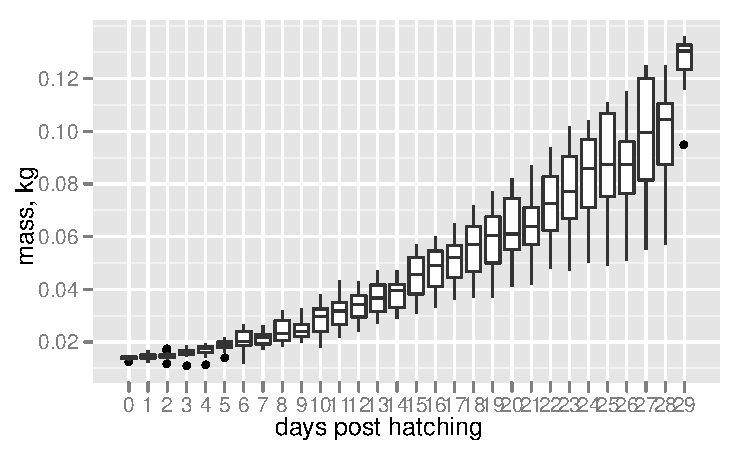
\includegraphics{figures/chukar-mass-boxplot.pdf}
\end{center}
\caption{Boxplot of chukar mass versus age. Explain what symbols are. Might be good to turn x-axis labels to avoid crowding.}
\label{fig:1mass}
\end{figure}

\subsection{Overall descent metrics}
\subsection{Onset of directed aerial descent}
\subsection{Inertial contribution to turns}


\section{Discussion}
\label{sec:1discussion}
Write discussion here. 

%\subsection{Evolutionary significance for the origins of bird flight}
%Birds lack a massive tail (unlike geckos) and their axial skeleton is stiffened by imbricated ribs and by the widespread fusion at the synsacrum (unlike mammals).  I would expect the avenues available to other vertebrate taxa for generating zero-angular-momentum turns are not present in birds, and dynamic models based on these other taxa should fail to predict the observed kinematics unless aerodynamic terms related to the wings or legs are added.  To test this further, patches could be used to augment areas (to simulate plumage changes with size held constant).  
%
%Theropod ancestors of birds had similar hips but lacked the rib cage stiffening; they also possessed long tails, and studies of falling bird chicks alone may not fully address this.  I may wish to test this further by manipulations to increase tail inertia by adding a boom similar to a theropod tail, or by testing aerial righting reflexes in other archosaurs (caimans).  This would provide a (somewhat weak) extant phylogenetic bracket for the presence of aerial righting in bird ancestors.
%
%The size-scaling of aerial righting ability may also be informative.  Many phylogenetic reconstructions of size in the clades leading to birds suggest they were small, perhaps small enough that both inertia and aerodynamics are important in the initial aerial righting given the phylogenetic constraints on axial body movement.  


\section{Acknowledgements}
We thank Dylan Marks for his assistance with filming.  We thank Luis Guillen and Kathy Moorhouse for their advice and assistance in raising birds.  We thank the Berkeley Center for Integrative Biomechanics Education and Research for the use of high speed cameras.  We thank Lindsay Waldrop, Kelly Dorgan, Yonatan Munk, Yu Zeng, Erica Kim, Marc Badger, Sofia Chang, Nir Sapir, Victor Ortega, and Marta Wolf for their analysis suggestions, assistance and support.  DE was supported by an NSF IGERT Fellowship and by a grant from the National and Berkeley local chapter of Sigma Xi.

\index{maneuvering during ontogeny|)}

% \bibliography{references/chukar} % copy all citations from this to main bibliography


